\documentclass{beamer}
% \usepackage{multirow}
% \usepackage[backend=biber]{biblatex}
% \addbibresource{sample-base}
% \bibliography{}
\usetheme{Boadilla}
\title[C2SG Research Group]{Identifying Influences: A Machine Learning and Explainable AI Approach to Analyzing Social Media Addiction Resulting from Academic Frustration}
% \subtitle{Using Beamer}
% \author{NSysS 2024}
\author[Rofi, Eshita, Ahmed, Noor]{Ishmam~Bin~Rofi\inst{1}\inst{2}\and Mashiyat~Mahjabin~Eshita\inst{1}\inst{2}\and Md.~Sabbir~Ahmed\inst{1}\and Jannatun~Noor\inst{1}\inst{2}}
\institute[BracU]{\ins{1}Brac~University \and \ins{2}The~Computing~for~Sustainability~and~Social~Good~(C2SG)~Research~Group}
\date{21 December 2024}
\logo{
\includegraphics[height=1cm]{NSysS-2017-4th-logo-latest-300x290.jpg}}
% \logo{
\includegraphics[height = 1cm]{c2sghhh.jpg}}
% \logo{
%     \begin{minipage}[t]{0.3\textwidth}
%         
\includegraphics[width=0.5]{c2sghhh.jpg} % First logo (left)
%     \end{minipage}%
%     \hfill
%     \begin{minipage}[t]{0.3\textwidth}
%         
\includegraphics[height=1cm]{NSysS-2017-4th-logo-latest-300x290.jpg} % Second logo (right)
%     \end{minipage}
% }
% \AtBeginSection[]
% {
%   \begin{frame}
%     \frametitle{Table of Contents}
%     \tableofcontents[currentsection]
%   \end{frame}
% }
\begin{document}
% \begin{frame}
%     % \centering
%     % % Title
%     % {\Large \textbf{Identifying Influences:}}\\
%     % {\Large \textbf{A Machine Learning and Explainable AI Approach to Analyzing Social Media Addiction Resulting from Academic Frustration}}\\[0.5cm]
    
%     % % Authors and Institution
%     % \textbf{Authors:}\\
%     % Ishmam Bin Rofi, Mashiyat Mahjabin Eshita, Md. Sabbir Ahmed, Jannatun Noor\\[0.5cm]
    
%     % \textbf{Institution:}\\
%     % C2SG Research Group, BRAC University\\[1cm]
    
%     % % Logos
%     % 
\includegraphics[width=1.5cm]{NSysS-2017-4th-logo-latest-300x290.jpg} \hspace{1cm} % Conference logo
%     % 
\includegraphics[width=1.5cm]{c2sghhh.jpg} % Lab logo
%     % % \hspace{1cm}
%     % % 
\includegraphics[width = 1.5cm]{bracu.png}
%     \maketitle
% \end{frame}



\begin{frame}
        \maketitle
\end{frame}

\begin{frame}
    % Table of contents
    \frametitle{Table of Contents}
    \tableofcontents % Automatically generated based on \section commands
\end{frame}

\section{Motivation Behind The Work}

\begin{frame}{Motivation}

\begin{figure}
    \centering
    \begin{minipage}{0.25\linewidth}
        \centering
        \includegraphics[width=\linewidth]{student academic frustrated.pdf}
        % \caption*{(a) LIME Interpretation of the XGBoost Model's Predictions}
    \end{minipage}
    \hfill
    \begin{minipage}{0.25\linewidth}
        \centering
        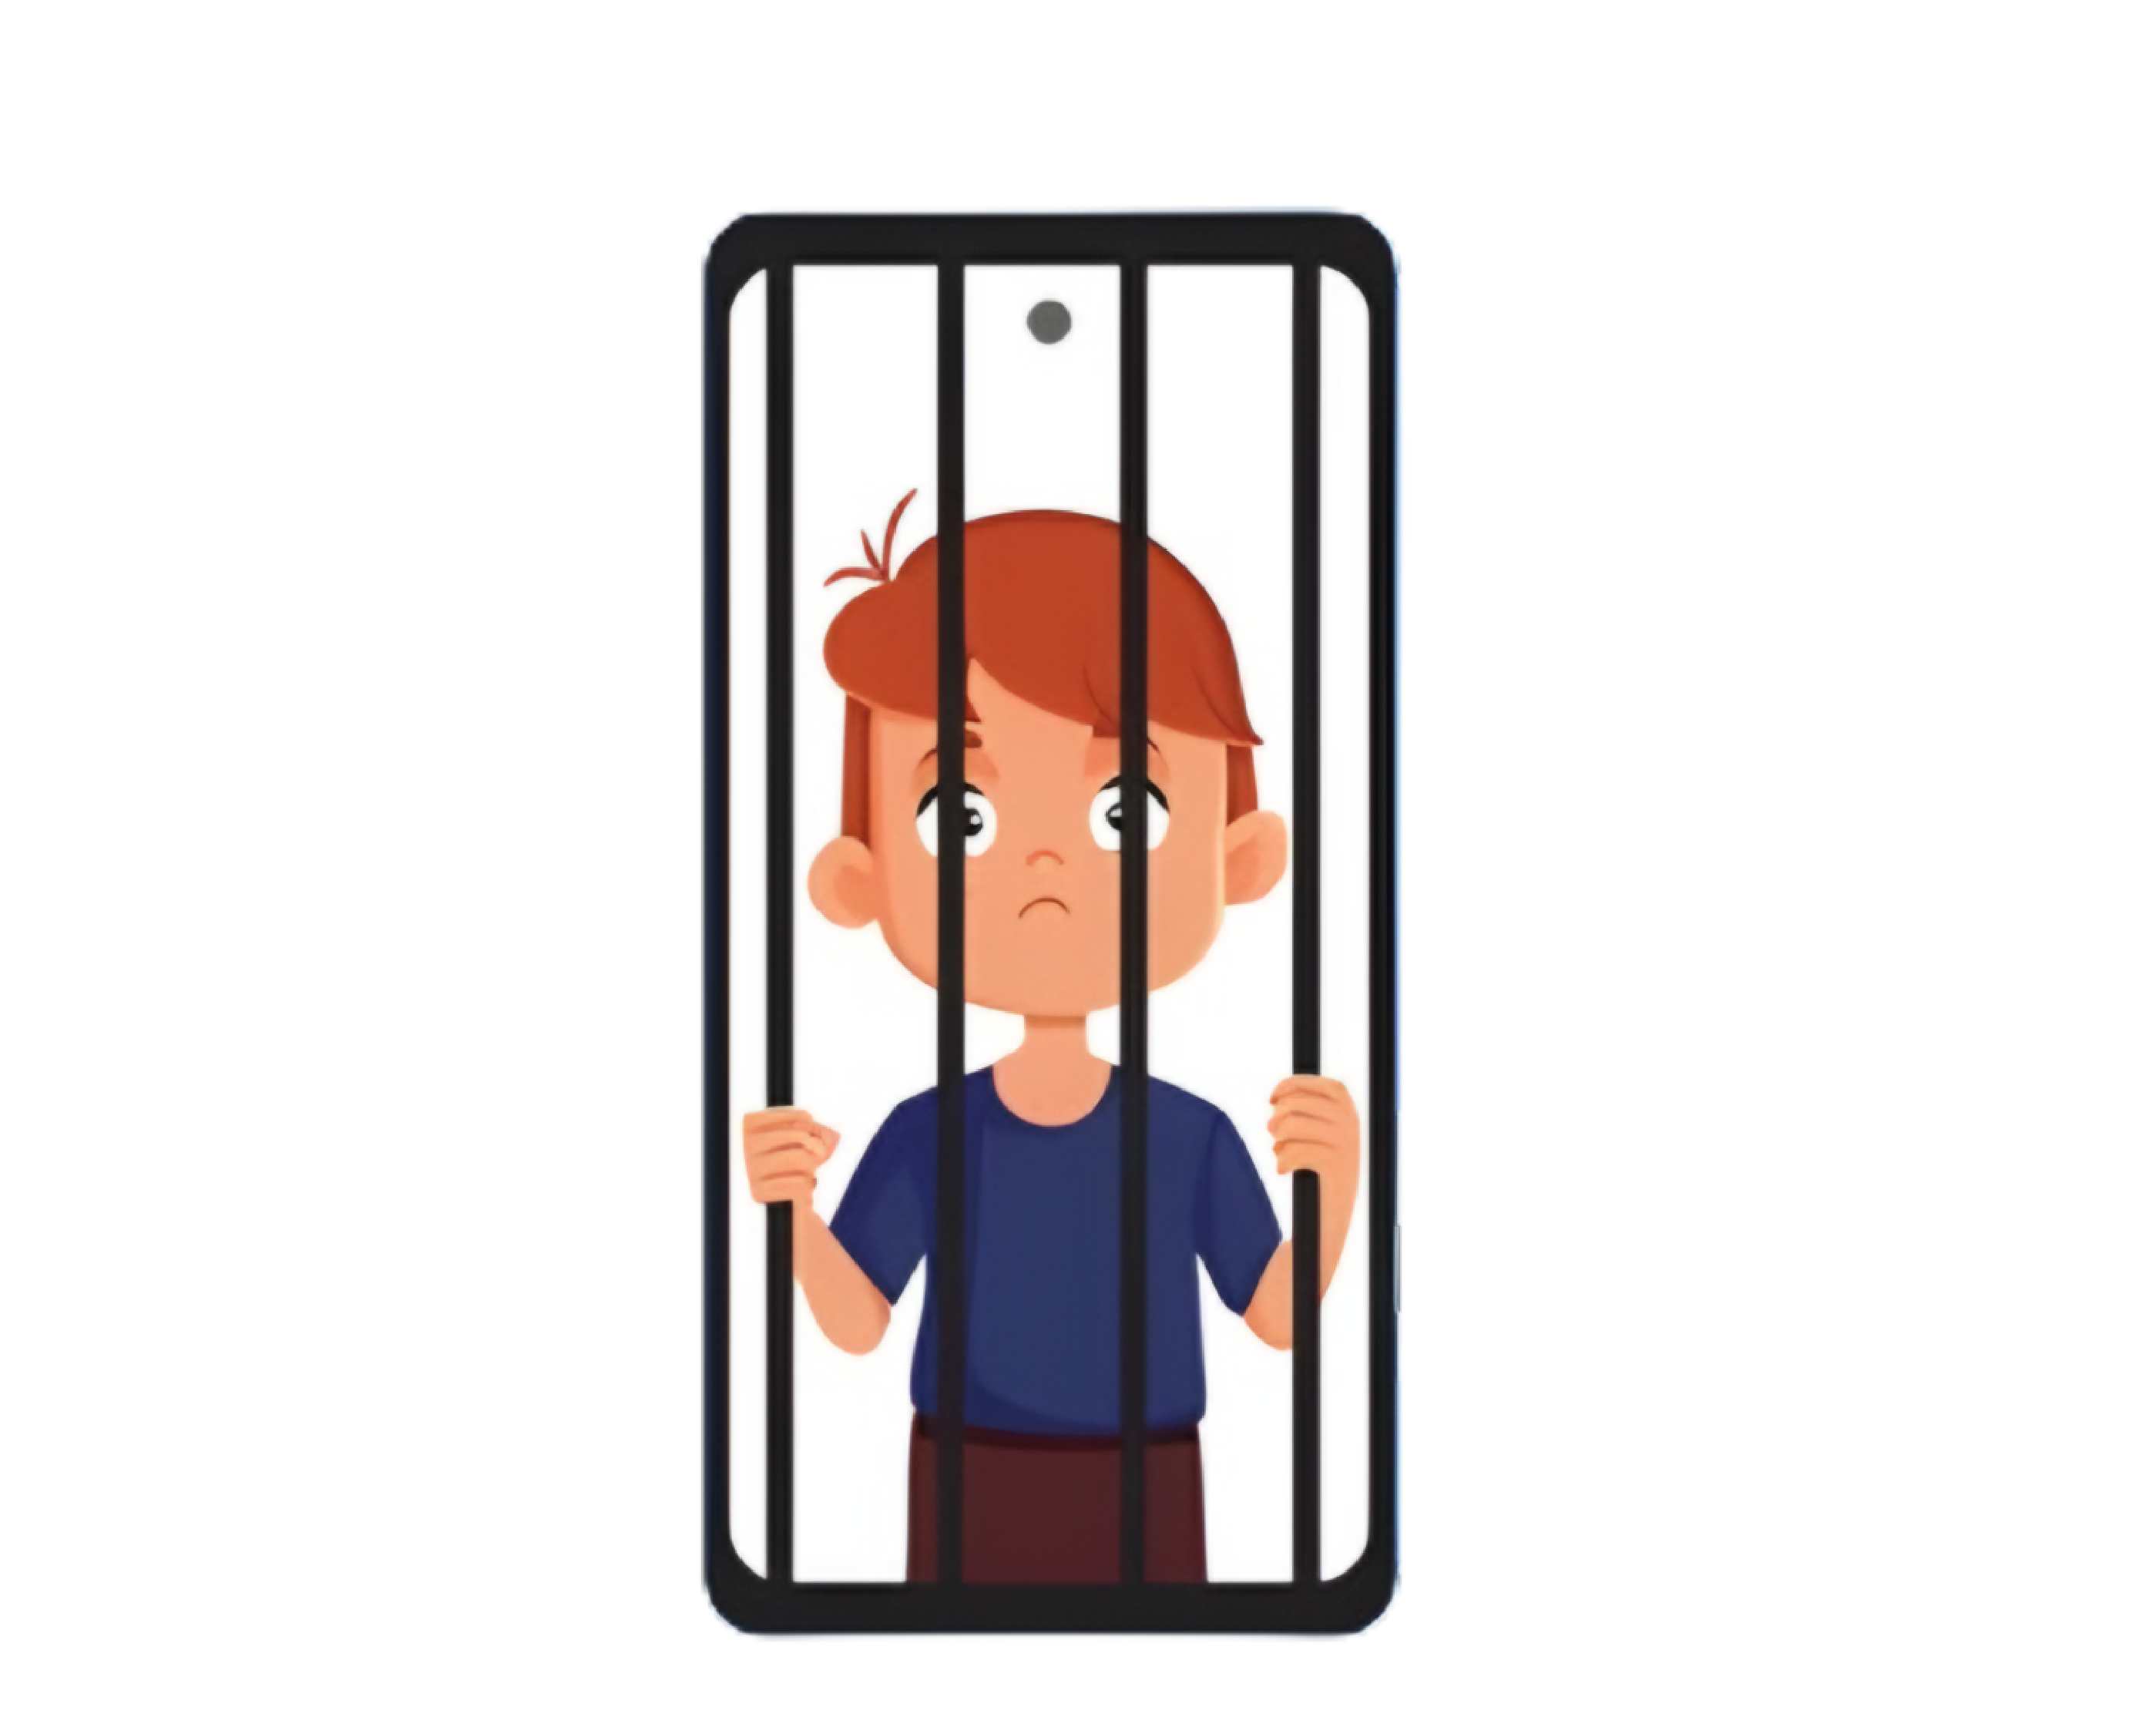
\includegraphics[width=\linewidth]{phone addicted.pdf}
        % \caption*{(b) LIME Interpretation on Another Instance of the XGBoost Model's Predictions}
    \end{minipage}
    \caption{A reverse approach: Tracing Back Social Media addiction.}
    \label{fig:lime-comparison}
\end{figure}

    % \begin{itemize}
        \textbf{Why This Study?}
        \begin{itemize}
            \item Social media addiction is commonly seen as the cause of academic dissatisfaction, but \textbf{we explore the reverse relationship}: academic dissatisfaction driving social media addiction.
            \item Rising \textbf{dependency on social media} among students impacts mental health, productivity, and academic outcomes.
            % \item \textbf{Personalized Insights}: Using LIME, we identify individual drivers of addiction for actionable, tailored interventions.
            \item Relevant in a \textbf{post-pandemic world}, where social media usage among students has surged.
        \end{itemize}
    % \end{itemize}
\end{frame}


\section{Introduction}
\begin{frame}{Introduction}
    \begin{itemize}
        \item Social media addiction has become a significant concern, especially among students, driven by academic frustration.
        \item This paper explores the influence of academic dissatisfaction on social media addiction using a machine learning and explainable AI approach.
        \item The goal is to identify the key factors behind this addiction and provide insights for mitigating its impact.
    \end{itemize}
    \vfill % Push content to the top
    % \hspace*{-.5cm} % Adjust horizontal alignment
    % \vspace*{-2.5cm}
    % 
\includegraphics[width=1.5cm]{NSysS-2017-4th-logo-latest-300x290.jpg} % Insert conference logo
\end{frame}

\section{Literature Review}
\begin{frame}{Literature Review}

\textbf{Existing Research:}
\begin{itemize}
    \item Social media platforms significantly affect students' academic success:
    \begin{itemize}
        \item Ramzan et al. (2023) discussed how ESL students use social media to enhance academic performance and engagement [1].
        \item Fukubayashi and Fuji (2021) highlighted the link between excessive social media use, social comparison, and career frustration [2].
        \item Iwamoto and Chun (2020) examined the emotional ramifications of overuse, including depression, anxiety, and stress in students [3].
    \end{itemize}
\end{itemize}

\textbf{Research Gaps:}
\begin{itemize}
    \item While much research assumes social media addiction leads to academic dissatisfaction, Mohamed et al. (2019) explored the opposite relationship but lacked machine learning insights [4].
    \item Few papers utilize \textbf{machine learning and explainable AI} to identify actionable, personalized insights.
\end{itemize}

\end{frame}


\section{Methodology of Our Work}
\begin{frame}{Methodology}
    \begin{itemize}
        \item \textbf{Data Collection:} Data was collected from diverse universities using surveys distributed through social media and in-person visits, focusing on academic frustration and social media usage patterns.
        \item \textbf{Machine Learning Models:} XGBoost, KNN, and Gradient Boosting were employed to predict social media addiction. Each was chosen for their strengths in handling structured data and capturing complex patterns.
        \item \textbf{Explainable AI:} LIME was applied for instance-level interpretability, helping identify personalized factors influencing social media addiction for targeted interventions.
    \end{itemize}
\end{frame}


\begin{frame}{Workflow}
\begin{figure}
        \centering
        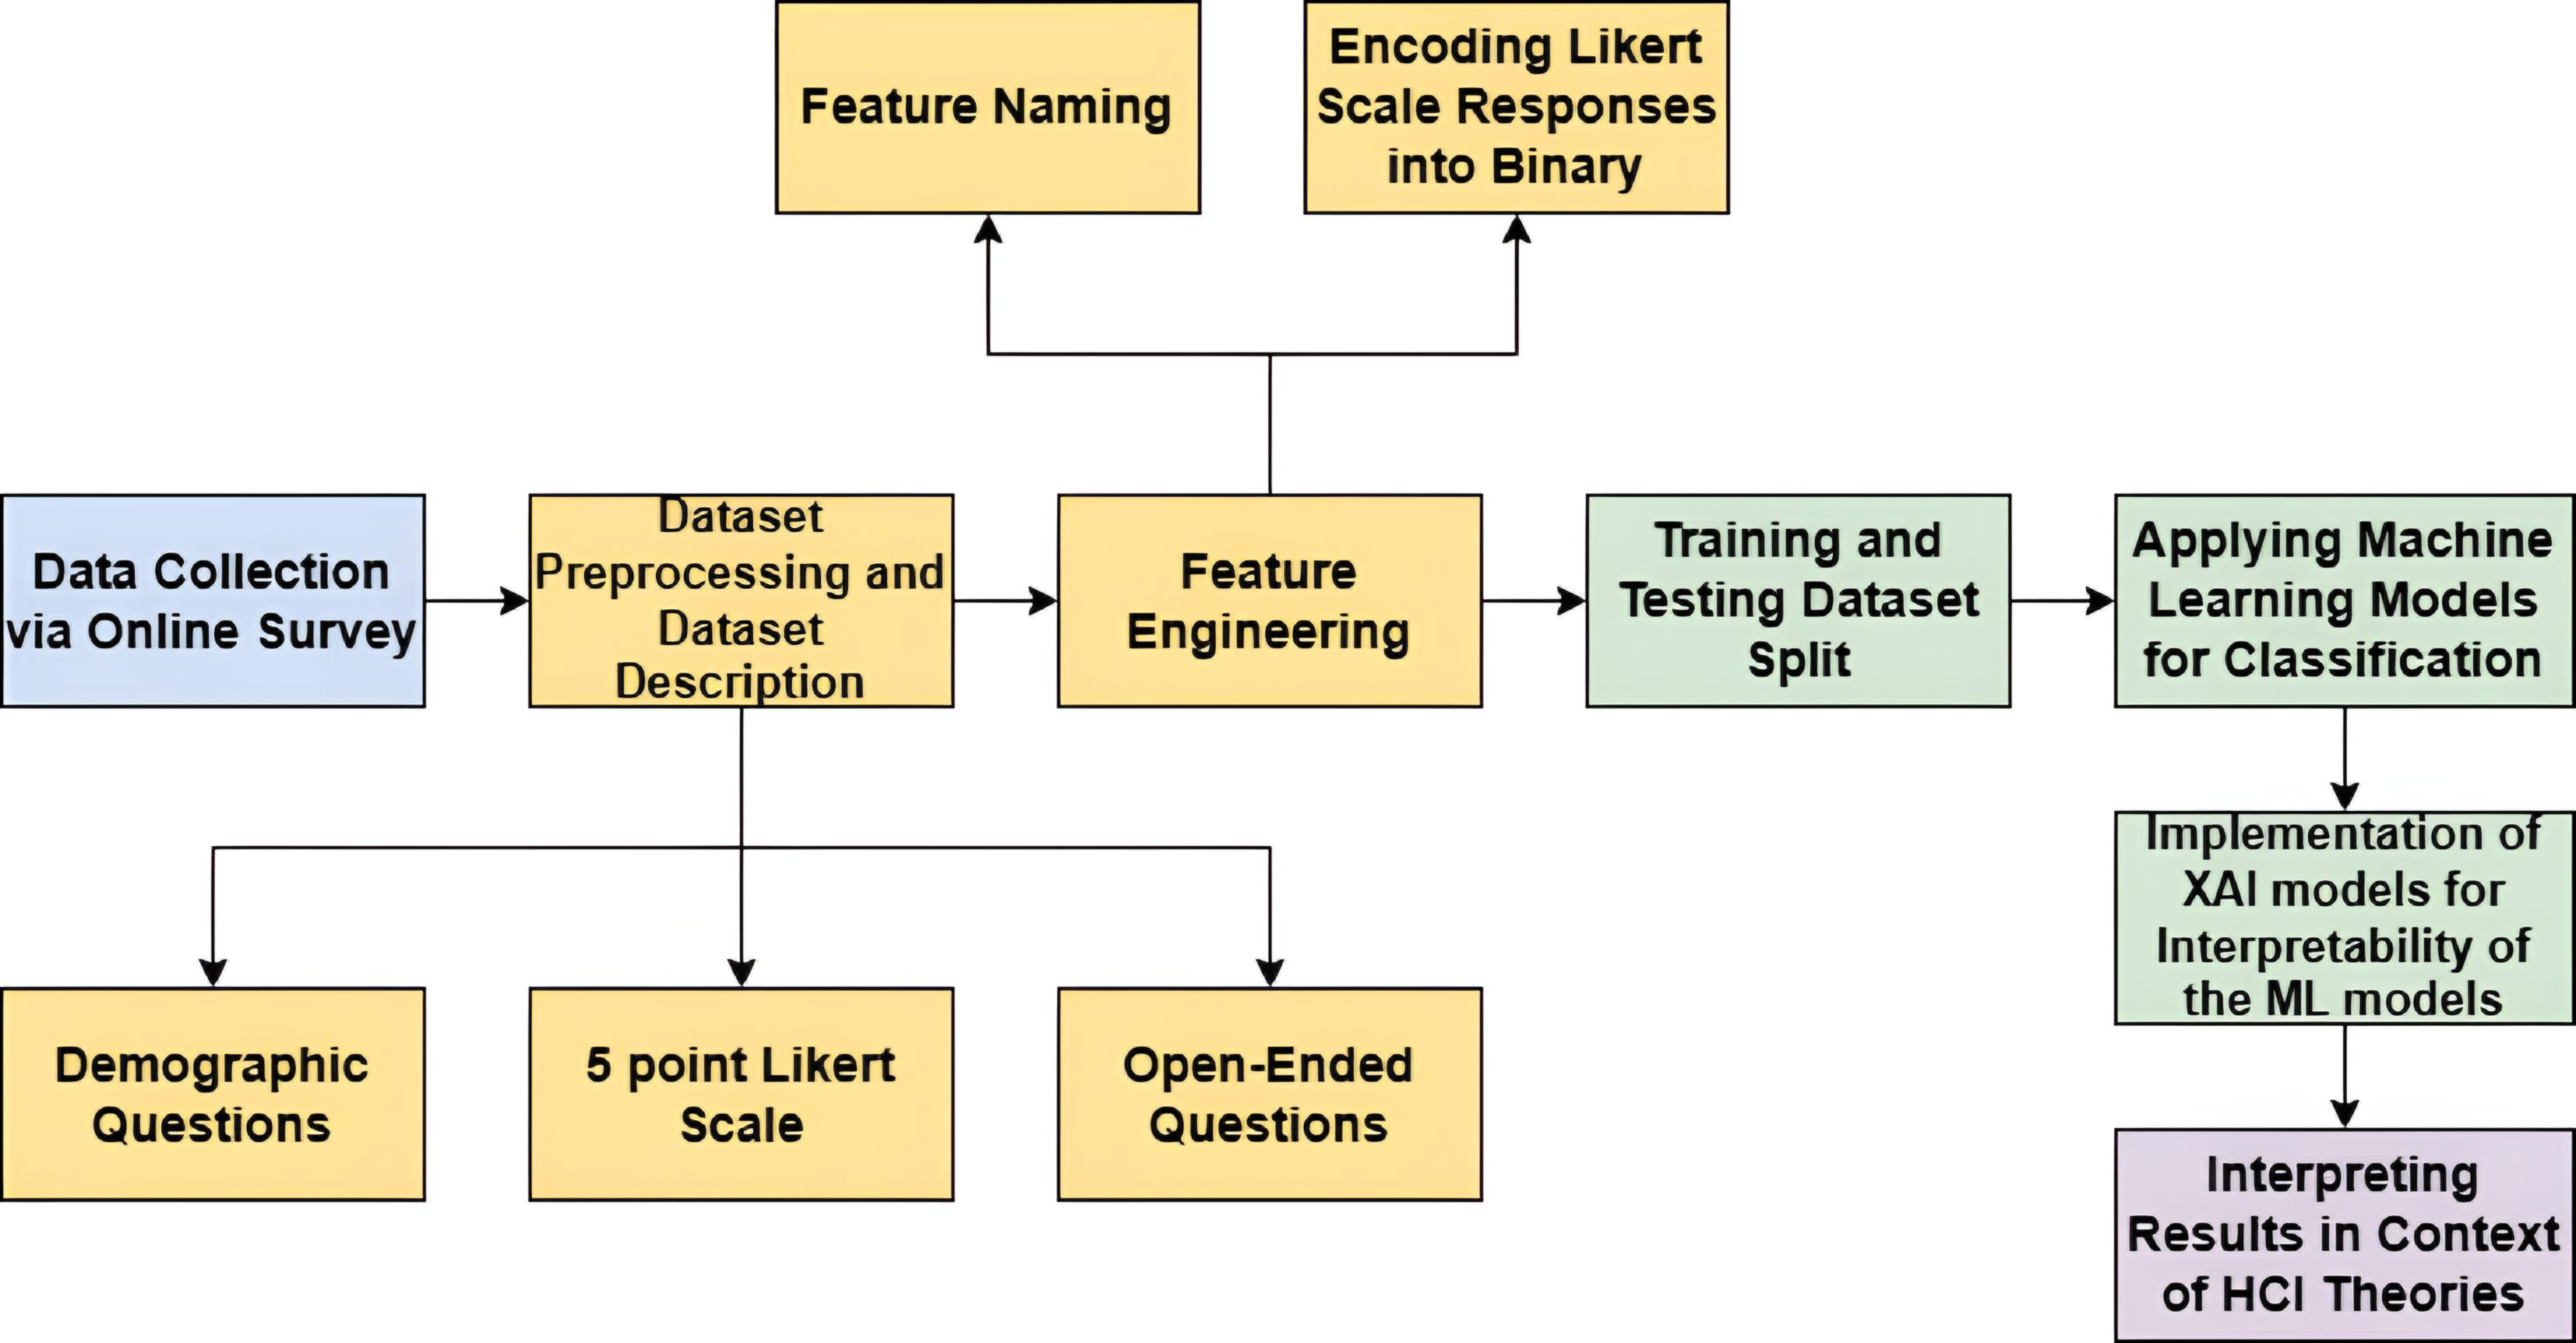
\includegraphics[width=0.7\linewidth]{workflow.pdf}  % Adjust the path and size as needed
        \caption{Workflow of our study}
    \end{figure}
\end{frame}

\begin{frame}{Dataset Collection and Processing}
    \begin{itemize}
        \item \textbf{Data Collection:}
        \begin{itemize}
            \item Conducted over a period of \textbf{2 months} (15 October 2023 to 12 December 2023).
            \item Targeted university students from \textbf{Bangladesh}.
            \item Data was collected using Google Forms distributed via social media, Messenger groups, and in-person classroom visits.
            \item Total data points collected: \textbf{943}.
        \end{itemize}

        \item \textbf{Dataset Composition:}
        \begin{itemize}
            \item Undergraduate students: \textbf{897}.
            \item Graduate students: \textbf{46}.
            \item Gender distribution: 
            \begin{itemize}
                \item Male: \textbf{593}, Female: \textbf{341}, Prefer not to disclose: \textbf{9}.
            \end{itemize}
        \end{itemize}
    \end{itemize}
\end{frame}


\begin{frame}{Dataset Collection and Processing (Contd.)}
\begin{figure}
    \centering
    \begin{minipage}{0.48\linewidth}
        \centering
        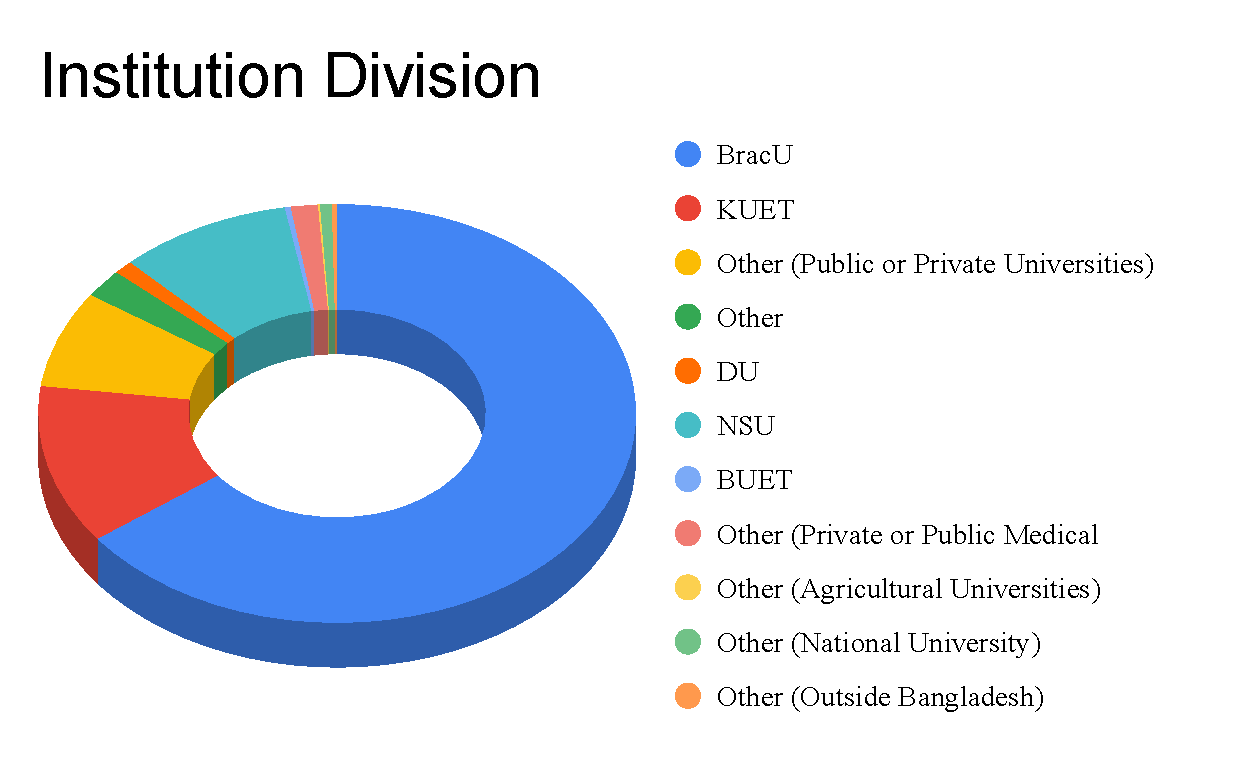
\includegraphics[width=\linewidth]{Institution Division.pdf}
        \caption{Description of Institutions of our Data Collection}
        \label{fig: Institution}
    \end{minipage}
    \hfill
    \begin{minipage}{0.48\linewidth}
        \centering
        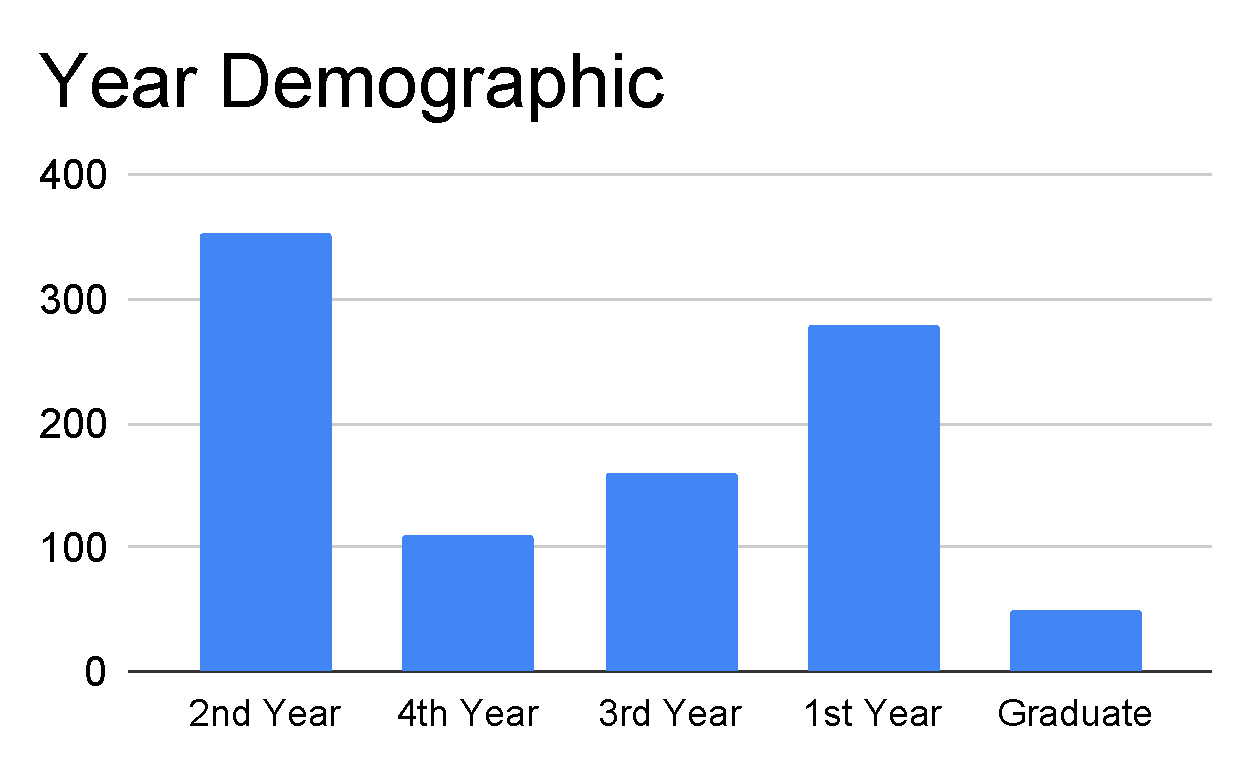
\includegraphics[width=\linewidth]{Year Demographic.pdf}
        \caption{Division of Student's Years}
        \label{fig:Year}
    \end{minipage}
\end{figure}
\end{frame}

\begin{frame}{Dataset Collection and Processing (Contd.)}
    \begin{itemize}
        \item \textbf{Data Validation:}
        \begin{itemize}
            \item Ensured reliability by applying \textbf{conflict analysis} to check consistency.
            \item \textbf{Cronbach's Alpha} scored at 82.07\%, confirming the internal consistency and reliability of the Likert-scale items.
        \end{itemize}
        
        \item \textbf{Data Preprocessing Steps:}
        \begin{enumerate}
            \item \textbf{Removed Noise:} Filtered out any redundant or conflicting responses through systematic checks.
            \item \textbf{Likert Scale Conversion:} Standardized the scale responses for uniformity.
            \item \textbf{Feature Engineering:} Renamed lengthy feature names to concise ones for improved interpretability in machine learning models.
            \item \textbf{Normalization:} Applied scaling techniques to ensure the data range consistency for ML models.
        \end{enumerate}

        \item \textbf{Dataset Integrity:} Maintained no missing values post-validation.
    \end{itemize}
\end{frame}





\section{Results}
\begin{frame}{Results: Machine Learning}
    \begin{itemize}
        \item \textbf{Model Performance:}
        The XGBoost model achieved an accuracy of 85\%, with a precision of 80\%, recall of 95\%, and an F1-score of 87\%.
        
        \item \textbf{Key Findings:}
        Academic stress, lack of social support, and excessive time spent on academic tasks were identified as the most influential factors predicting social media addiction.
        
        \item \textbf{Confusion Matrix:}
        The model performed effectively in identifying individuals at risk of social media addiction (Class 0), with minimal misclassification.
    \end{itemize}
\end{frame}


    % \begin{table}[h]
    %     \centering
    %     \begin{tabular}{|c|c|c|c|c|}
    %         \hline
    %         \textbf{Model} & \textbf{Accuracy} & \textbf{Precision} & \textbf{Recall} & \textbf{F1-Score} \\
    %         \hline
    %         Model 1 & 85\% & 0.83 & 0.88 & 0.85 \\
    %         Model 2 & 82\% & 0.80 & 0.84 & 0.82 \\
    %         Model 3 & 87\% & 0.85 & 0.89 & 0.87 \\
    %         \hline
    %     \end{tabular}
    %     \caption{Machine Learning Model Performance}
    % \end{table}
\end{frame}

\begin{frame}{Results: Machine Learning (Contd.)}
\begin{table}[]
\centering
\caption{Performance Metrics of the Machine Learning Models}
\label{tab:Metrics}
\begin{tabular}{|c|cccc|}
\hline
Model                           & \multicolumn{4}{c|}{Performance Metrics}                                                                            \\ \hline
                                & \multicolumn{1}{c|}{Class} & \multicolumn{1}{c|}{Precision (\%)} & \multicolumn{1}{c|}{Recall (\%)} & F1 Score (\%) \\ \hline
\multirow{XGBoost}       & \multicolumn{1}{c|}{0}     & \multicolumn{1}{c|}{80}             & \multicolumn{1}{c|}{95}          & 87            \\ \cline{2-5} 
                                & \multicolumn{1}{c|}{1}     & \multicolumn{1}{c|}{57}             & \multicolumn{1}{c|}{21}          & 31            \\ \hline
\multirow{KNN}            & \multicolumn{1}{c|}{0}     & \multicolumn{1}{c|}{83}             & \multicolumn{1}{c|}{88}          & 85            \\ \cline{2-5} 
                                & \multicolumn{1}{c|}{1}     & \multicolumn{1}{c|}{42}             & \multicolumn{1}{c|}{34}          & 38            \\ \hline
\multirow{Gradient Boost} & \multicolumn{1}{c|}{0}     & \multicolumn{1}{c|}{81}             & \multicolumn{1}{c|}{89}          & 85            \\ \cline{2-5} 
                                & \multicolumn{1}{c|}{1}     & \multicolumn{1}{c|}{47}             & \multicolumn{1}{c|}{30}          & 37            \\ \hline
\end{tabular}
\end{table}
\begin{itemize}
    \item We particularly focus on the recall rate of class 0, which represents individuals dependent on social media due to dissatisfaction with their academic results.
    \item High recall ensures that we capture as many individuals in this category as possible.
\end{itemize}



\end{frame}

\begin{frame}{Results: Explainable AI (XAI)}
    \begin{itemize}
        \item \textbf{Local Explanations (Why Local Explanations Matter):}
        \begin{itemize}
            \item Our focus is on understanding individual students to provide personalized insights.
            \item LIME’s local explanations reveal the specific combination of factors driving addiction for each student.
        \end{itemize}

        % \item \textbf{Examples:}
        % \begin{itemize}
        %     \item \textbf{Student A:} Procrastination and peer comparison are key drivers of social media addiction.
        %     \item \textbf{Student B:} Low academic performance is the primary factor influencing addiction.
        % \end{itemize}

        \item \textbf{Importance of Personalization:}
        \begin{itemize}
            \item By focusing on individual insights, we can:
            \begin{itemize}
                \item Identify unique needs of each student.
                \item Develop targeted interventions like counseling for procrastination or strategies for managing peer pressure.
            \end{itemize}
        \end{itemize}

        \item \textbf{Why Local Explanations Are Enough:}
        \begin{itemize}
            \item \textbf{Personalized Interventions:} Addressing social media addiction requires tailored solutions rather than one-size-fits-all strategies.
            \item \textbf{Actionable Insights:} Local explanations empower educators and counselors to understand and support each student's specific challenges.
        \end{itemize}
    \end{itemize}
\end{frame}


% \begin{frame}{Result: Explaiable AI}
%     \begin{figure}
%         \centering
%         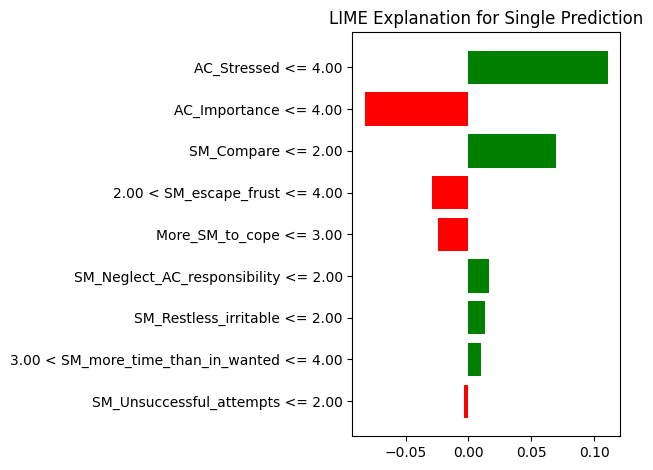
\includegraphics[width=0.7\linewidth]{lime.png}
%         \caption{LIME Interpretation of the XGBoost Model's Predictions}
%         \label{fig:enter-label}
%     \end{figure}
    
% \end{frame}

% \begin{frame}{Result: Explaiable AI (Contd.)}
%     \begin{figure}
%         \centering
%         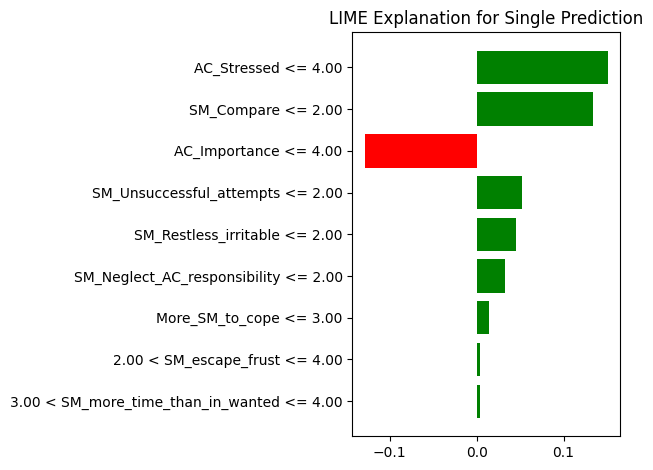
\includegraphics[width=0.7\linewidth]{new LIME.png}
%         \caption{LIME Interpretation on another instances of the XGBoost Model's Predictions.}
%         \label{fig:enter-label}
%     \end{figure}
% \end{frame}

\begin{frame}{Result: Explainable AI (Contd.)}
\begin{figure}
    \centering
    \begin{minipage}{0.48\linewidth}
        \centering
        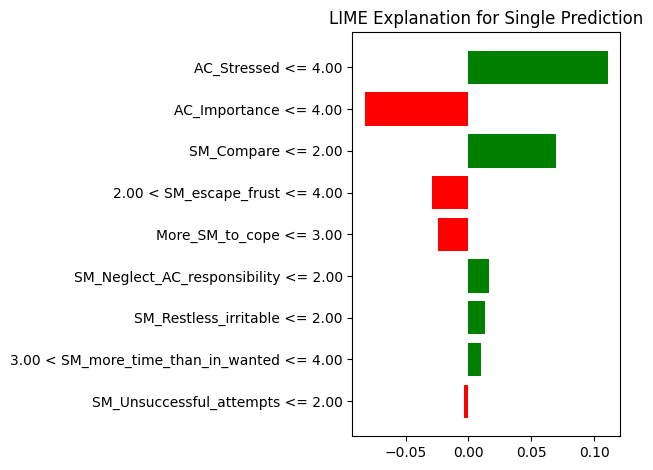
\includegraphics[width=\linewidth]{lime.png}
    \end{minipage}
    \hfill
    \begin{minipage}{0.48\linewidth}
        \centering
        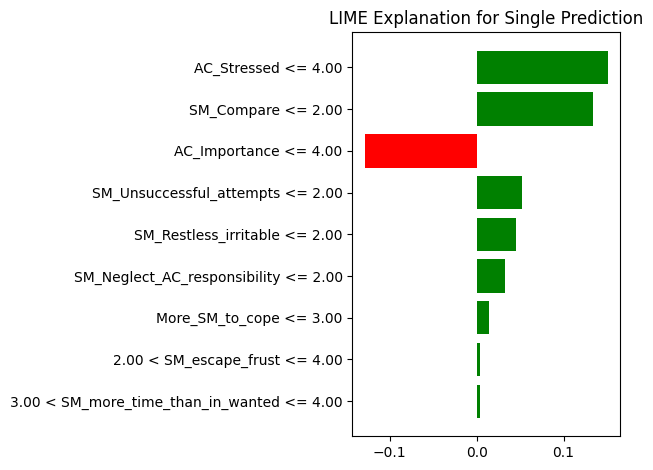
\includegraphics[width=\linewidth]{new LIME.png}

    \end{minipage}
    \caption{Comparative LIME Explanations for XGBoost Predictions}
    \label{fig:lime-comparison}
\end{figure}
\end{frame}




\section{Discussions}
\begin{frame}{Discussion}
    \begin{itemize}
        \item \textbf{Key Insights:}
        \begin{itemize}
            \item Academic dissatisfaction is a primary factor driving social media addiction among students.
            \item Behavioral traits like procrastination and stress amplify addiction risk.
        \end{itemize}
        
        \item \textbf{Implications:}
        \begin{itemize}
            \item Universities should focus on academic counseling to address dissatisfaction.
            \item Developing awareness programs to mitigate stress and unhealthy social media habits.
        \end{itemize}
    \end{itemize}
\end{frame}

\section{Limitations and Future Work}
\begin{frame}{Limitations and Future Work}
    \textbf{Limitations:}
    \begin{itemize}
        \item Data collected from limited universities in Bangladesh, restricting generalizability.
        \item Cross-sectional study design; cannot establish causation.
    \end{itemize}

    \textbf{Future Work:}
    \begin{itemize}
        \item Expanding data collection to a diverse demographic across more institutions.
        \item In another ongoing study of our research team, we are performing a qualitative study on leveraging social media platforms to help students overcome their addiction.
    \end{itemize}
    
\end{frame}

\begin{frame}{References}
% \bibliography{sample-base}
% \printbibliography
    \begin{enumerate}
        
    % \end{enumerate}
        \item Ramzan, M., Bibi, R., \& Khunsa, N. (2023). Unraveling the Link between Social Media Usage and Academic Achievement among ESL Learners: A Quantitative Analysis. \textit{Global Educational Studies Review, VIII}(2023), 407–421.
        \item Fukubayashi, N., \& Fuji, K. (2021). Social comparison on social media increases career frustration: A focus on the mitigating effect of companionship. \textit{Frontiers in Psychology, 12}(2021), 720960.
        \item Iwamoto, D., \& Chun, H. (2020). The emotional impact of social media in higher education. \textit{International Journal of Higher Education, 9}(2), 239–247.
        \item Mohamed, S., Sidek, S., Izharrudin, S. Z., Kudus, N., Hassan, M. A., \& Noor, M. A. (2019). Social Media Usage and Its Impact on Work Productivity at a Malaysian University. \textit{International Journal of Recent Technology and Engineering (IJRTE), 8}(2019), 167–172.
    \end{enumerate}
\end{frame}



\begin{frame}
    \begin{center}
        \Huge Thank You! \\
        \vspace{1cm}
        \Large Any Questions? \\
        \vspace{0.5cm}
        % \textbf{}
        
\includegraphics[width=0.2\textwidth]{c2sghhh.jpg} % Optional: Add your logo here
    \end{center}
\end{frame}

\begin{frame}{Extension}
    
\end{frame}

\end{document}


